\begin{frame}{$d(K^-, p)"\pi^-\Lambda"$ and $d(K^-, p)"\Sigma^0"$ Cross Section}
  \begin{tabular}{ccc}
    \begin{minipage}{0.25\hsize}
      \begin{figure}
        \scriptsize
        Event Num
        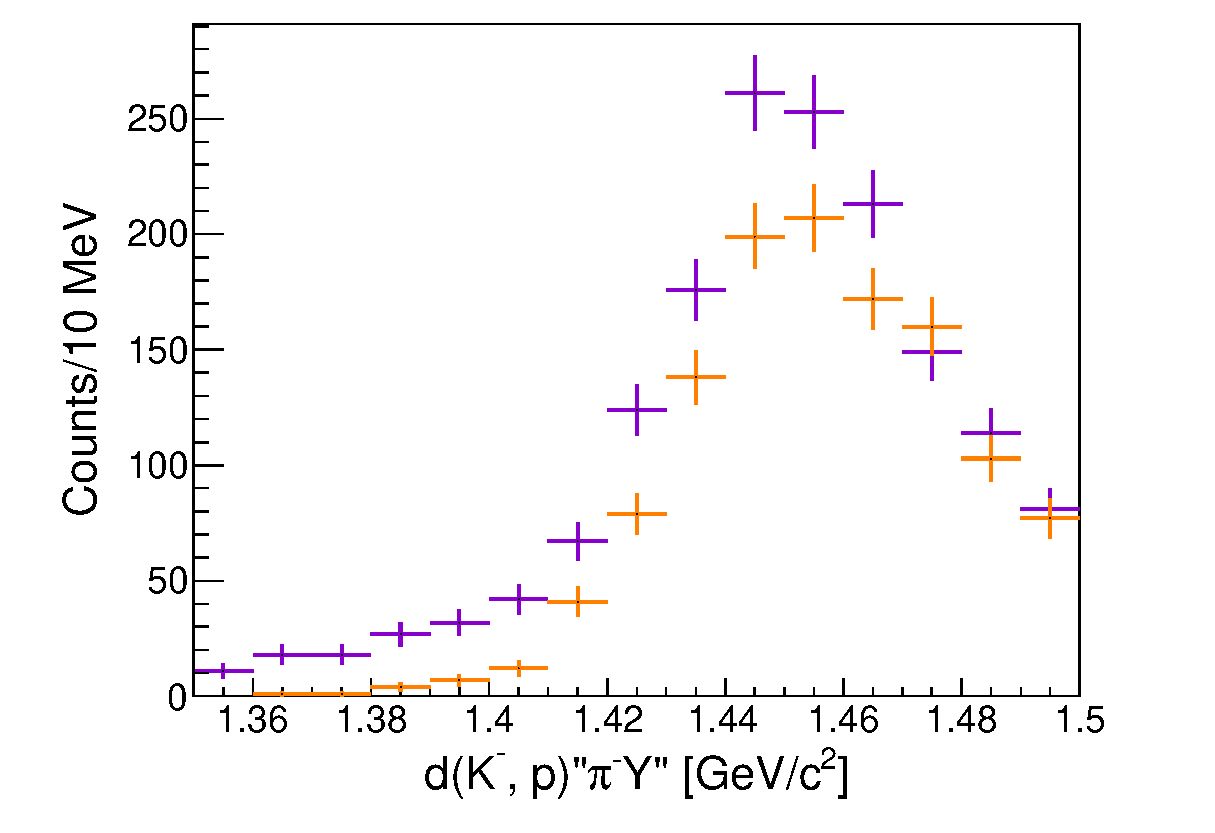
\includegraphics[width=3cm]{../pic/Run68/KP_ana/KP_MM_pimY.eps}
      \end{figure}      
    \end{minipage}
    \begin{minipage}{0.25\hsize}
      \begin{figure}
        \scriptsize
        Acceptance
        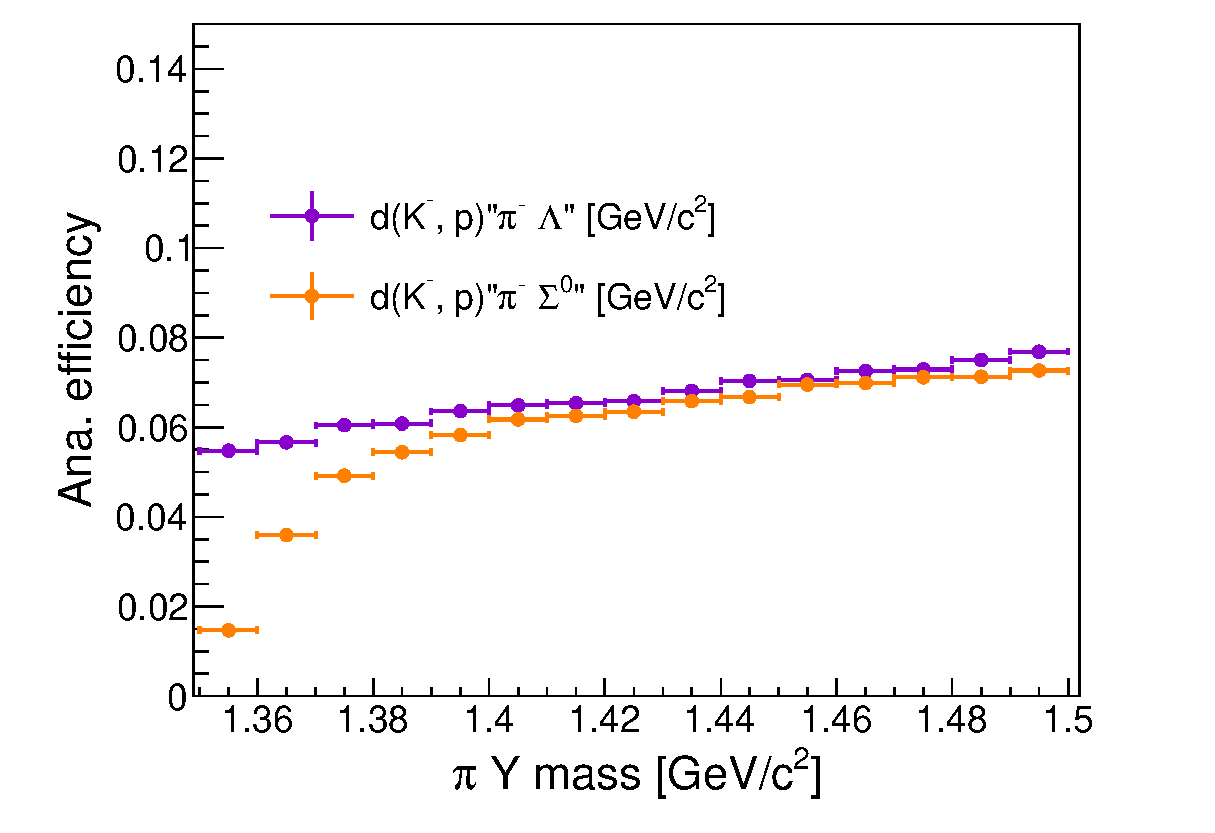
\includegraphics[width=3cm]{../pic/Run68/KP_ana/kp_acc.eps}
      \end{figure}      
    \end{minipage}    
    \begin{minipage}{0.5\hsize}
      \scriptsize
      Left figure shows event number selected \\ by before page.\\
      Down two figure represent converted CS.\\
      Boxes indicate statisical error.\\
      Error bar includes scaling factor error.
    \end{minipage}
  \end{tabular}
  \begin{tabular}{cc}
    \begin{minipage}{0.5\hsize}
      \begin{figure}
        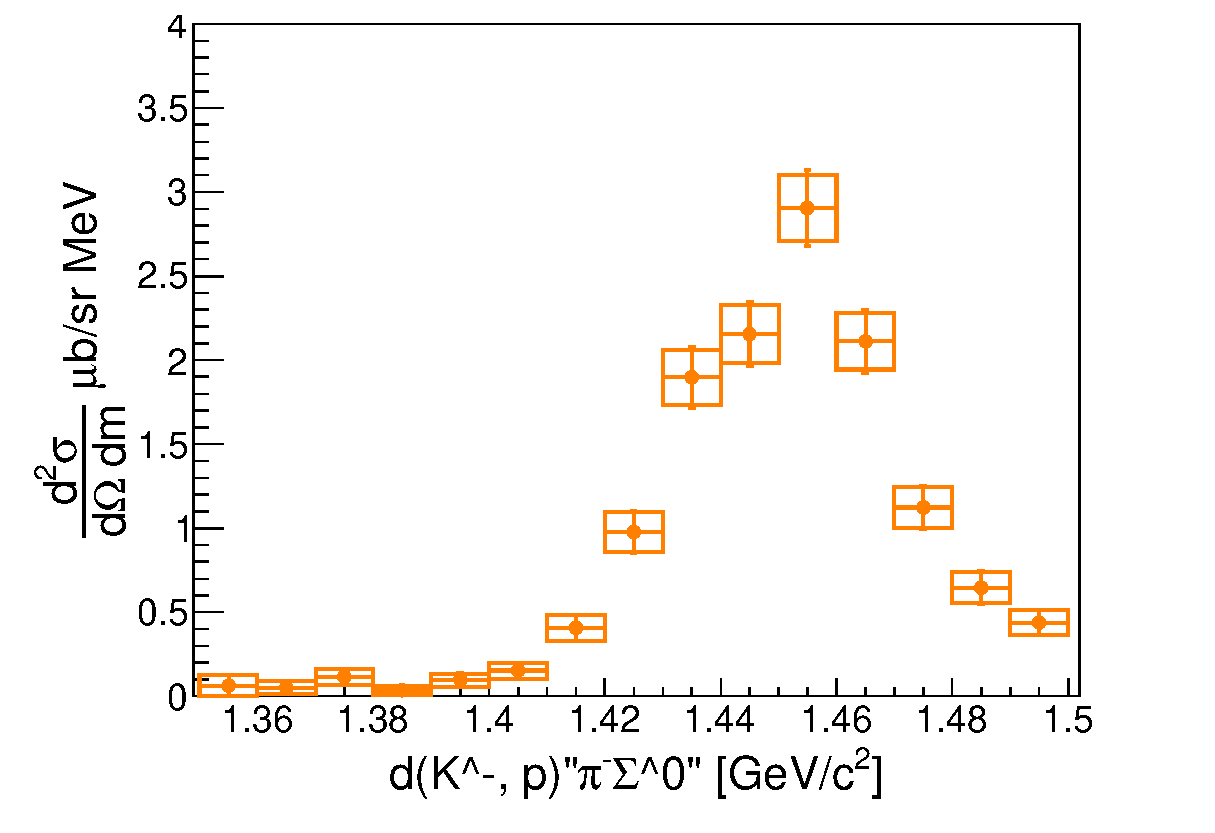
\includegraphics[width=5cm]{../pic/Run68/KP_ana/pimS0_CS_zoom.eps}
      \end{figure}
    \end{minipage}

    \begin{minipage}{0.5\hsize}
      \begin{figure}
        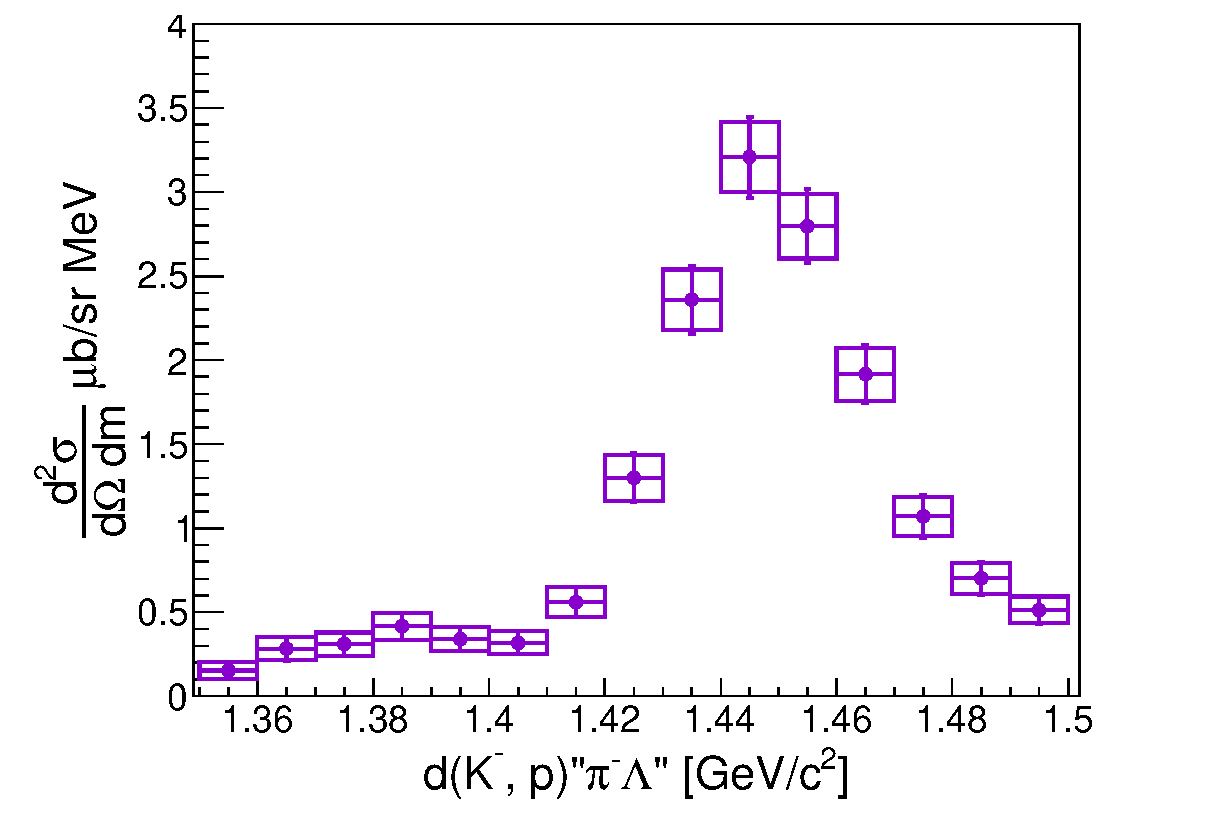
\includegraphics[width=5cm]{../pic/Run68/KP_ana/pimL_CS_zoom.eps}
      \end{figure}
    \end{minipage}
  \end{tabular}
  \centering
  I=1 scattering amplitude was suppressed below the $\bar{K}N$ threshold.
\end{frame}
